\documentclass{beamer}
\def\java{\texttt{Java}}
\def\mytoday{26 October 2016}
\usepackage{pgfpages}\def\mpause{\pause}
%\usepackage{pgfpages}\pgfpagesuselayout{8 on 1}[a4paper,border shrink=1mm, landscape]\def\mpause{}
\usepackage{url}
\usepackage{verbatim}
\usepackage{color}
\usepackage{listings}
\usepackage{code}
\usepackage{textcomp}

%\usepackage{bm}
\usepackage{beamerthemesplit}
\defbeamertemplate*{footline}{infolines theme}{
\hspace*{2ex}    \insertframenumber{} / \inserttotalframenumber\hspace*{2ex} 
\copyright Manfred Kerber
%   \insertpagenumber{} / \insertpresentationendpage \hspace*{2ex}
  \vskip1ex}

\def\mcolor#1#2{\rule{0ex}{0ex}\color{#1}#2\color{black}{}}
\usetheme{Copenhagen}
%\setbeamercolor{title}{fg=red!80!black,bg=red!20!white}\def\mpause{\pause}
\makeatletter % code block to allow custom labels to be cross-ref'ed; see comp.text.tex "customized display labels cross-ref'd" 

\begin{document}

\title{MSc/ICY Software Workshop\\
Testing (Revisited)\\Functions\\Interfaces}

\author[Manfred~Kerber]{\begin{tabular}{ll}
\mcolor{blue}{Manfred Kerber} &   {\tt www.cs.bham.ac.uk/\~{}mmk}\\
\end{tabular}}

\date{\mytoday}

\begin{frame}
\titlepage
\end{frame}

\begin{frame}
\frametitle{Testing}
(partly based on material by Christoph Lange and Chris Bowers)\bigskip

\mcolor{blue}{\textbf{How to test?}}\bigskip

\begin{itemize}
\item All the code should be covered by tests
      (e.g.\ both branches of an if-then-else).
\item You should test sufficiently many \textit{typical} cases.
\item You should test border cases (e.g.\ for an array
  \mcolor{blue}{\texttt{a}} whether \mcolor{blue}{\texttt{a[0]}} and
  \mcolor{blue}{\texttt{a[a.length-1]}} are properly
  initialized/changed).
\item You should write your code so that it is testable as far as
  possible (e.g., do not write a sophisticated print method since
  that cannot be tested by JUnit), but write a sophisticated \texttt{toString}
  method (since it can be tested by JUnit).
\end{itemize} % ends low level
\end{frame}

\begin{frame}
\frametitle{A quote by E. W. Dijkstra (2000)}
\begin{quote} % Dijkstra
  \mcolor{blue}{A programmer has to be able to demonstrate that his
    program has the required properties. If this comes as an
    afterthought, it is all but certain that he won't be able to meet
    this obligation only if he allows this obligation to influence his
    design, there is hope that he can meet it. Pure a posteriori
    verification denies you that wholesome influence and is therefore
    putting the cart before the horse.}
\end{quote}
\end{frame}

\begin{frame}
\frametitle{Test-Driven Development}
\begin{itemize}
\item Program by intent
\begin{enumerate}
\item Start by defining a set of test cases
\begin{itemize}
\item Pay attention to border cases!
\end{itemize}
\item Write code that passes the tests
\end{enumerate}

\item\small
%
\verbatiminput{stemmer.java}
\end{itemize} % ends low level
\end{frame}

\begin{frame}
\frametitle{Test-Driven Development (Cont'd)}

\begin{itemize}
\item Use tests as a template to create code
\item\ \\
\small
%
\verbatiminput{stemmerProg.java}
\end{itemize}

\mcolor{blue}{Find the right pattern to make defining test cases easier.}

\end{frame}

\begin{frame}
\frametitle{Unit testing}
\label{sec-9}
\begin{itemize}

\item \textbf{Unit} – small functional part of application that can be \textbf{tested independently}
\label{sec-9-1}%

\item A unit could be an \textbf{individual class or method}
\label{sec-9-2}%

\item A \textbf{set of test cases} are constructed to form a \textbf{test harness}\bigskip
\begin{center}
\label{sec-9-3}%
\includegraphics[width=.5\textwidth]{./bowers-test-harness.png}
\end{center}
\end{itemize} % ends low level
\end{frame}
\begin{frame}
\frametitle{JUnit testing with Eclipse}
\label{sec-10}
\begin{itemize}

\item JUnit: unit testing library for Java
\label{sec-10-1}%

\item Integrated into Eclipse/NetBeans/XCode/... IDEs
\label{sec-10-2}%

\item Separates source code from testing code
\label{sec-10-3}%

\item IDEs provide lots of nifty inspection tools
\label{sec-10-4}%

\item Well documented
\label{sec-10-5}%
\end{itemize} % ends low level
\end{frame}
\begin{frame}
\frametitle{Eclipse example}
\label{sec-11}

  Outline:
\begin{enumerate}
\item creating JUnit test
\item writing test cases
\item coding by intent
\begin{enumerate}
\item getting it wrong $\Rightarrow$ test fails
\item getting it right $\Rightarrow$ test passes
\end{enumerate}
\end{enumerate}
\end{frame}
\begin{frame}
\frametitle{Eclipse example: Creating JUnit test}
\label{sec-12}

\includegraphics[width=\textwidth]{./eclipse-junit-01-new-menu.png}
\end{frame}
\begin{frame}
\frametitle{Eclipse example (Cont'd): Creating JUnit test}
\label{sec-13}

\includegraphics[width=.5\textwidth]{./eclipse-junit-02-new-dialog.png}
\end{frame}
\begin{frame}
\frametitle{Eclipse example (Cont'd): Creating JUnit test}
\label{sec-14}

\includegraphics[width=.75\textwidth]{./eclipse-junit-03-methods.png}
\end{frame}
\begin{frame}
\frametitle{Eclipse example (Cont'd): Creating JUnit test}
\label{sec-15}

\includegraphics[width=\textwidth]{./eclipse-junit-04-build-path.png}
\end{frame}
\begin{frame}
\frametitle{Eclipse example (Cont'd): Creating JUnit test}
\label{sec-16}

\includegraphics[width=.75\textwidth]{./eclipse-junit-05-test-stub.png}
\end{frame}
\begin{frame}
\frametitle{Eclipse example (Cont'd): Writing test cases}
\label{sec-17}

\includegraphics[width=.75\textwidth]{./eclipse-junit-06-test-code.png}
\end{frame}
\begin{frame}
\frametitle{Eclipse example (Cont'd): Running a test}
\label{sec-18}

\includegraphics[width=.5\textwidth]{./eclipse-junit-07-run.png}
\end{frame}
\begin{frame}
\frametitle{Eclipse example (Cont'd): Running a test}
\label{sec-19}

\includegraphics[width=\textwidth]{./eclipse-junit-08-success.png}
\end{frame}
\begin{frame}
\frametitle{Eclipse example (Cont'd): Test-driven development}
\label{sec-20}

\includegraphics[width=\textwidth]{./eclipse-junit-09-tdd-test-first.png}
\end{frame}
\begin{frame}
\frametitle{Eclipse example (Cont'd): Test-driven development}
\label{sec-21}

\includegraphics[width=\textwidth]{./eclipse-junit-10-tdd-generate-code.png}
\end{frame}
\begin{frame}
\frametitle{Eclipse example (Cont'd): Test-driven development}
\label{sec-22}

\includegraphics[width=\textwidth]{./eclipse-junit-11-tdd-wrong-implementation.png}
\end{frame}

\begin{frame}
\frametitle{Eclipse example (Cont'd): Test-driven development}
\label{sec-23}

\includegraphics[width=.65\textwidth]{./eclipse-junit-12-tdd-test-failed.png}
\end{frame}

\begin{frame}[fragile]
\frametitle{JUnit assertions}
\label{sec-24}

\footnotesize
%\lstset{basicstyle=\ttfamily\scriptsize,columns=fixed,showstringspaces=false}

\begin{center}
\begin{tabular}{p{0.37\textwidth}p{0.62\textwidth}}
 Statement            &  What it does               \\\hline
\small\verb|fail() |
   &  Lets the test fail.  Useful for checking code\\
& is not reached under certain conditions.            \\
\small\verb|assertTrue(boolCond) |
   &  Checks that a condition is true                                                                 \\
\small\verb|assertEquals(expected,| &  Checks that two values are the same. Not a deep\\
\small\verb| actual, [tolerance]) | &   check, i.e., be careful with non-primitive values.  \\

\small\verb|assertArrayEquals| &  checks if two arrays are equal.\\
\small\verb| (expArray, actualArray)| & \\

\small\verb|assertNull(object)|
     &  Check that an object is null                                                                    \\
\small\verb|assertNotNull(object) |
   &  Check that an object is not null                                                                \\
\small\verb|assertSame(expected,|                 &  Check that both object references are the same.                                                 \\
\small\verb| actual)|             &\\
\small\verb|assertNotSame(expected,|              &  Check that both object references are not the same.                                             \\
\small\verb| actual)| &
\end{tabular}
\end{center}
\begin{itemize}

\item All methods take an optional first argument \textbf{message}.

\item Last argument tolerance for tests involving floating point numbers.
\end{itemize} % ends low level
\end{frame}

\begin{frame}\footnotesize
\frametitle{JUnit Assertions}
\verbatiminput{test1.java}
\end{frame}

\begin{frame}\renewcommand{\baselinestretch}{0.85}\small
\frametitle{JUnit Assertions (Cont'd)}
\verbatiminput{test2.java}
\end{frame}

\begin{frame}\small
\frametitle{JUnit Assertions (Cont'd)}
\verbatiminput{test3.java}
\end{frame}

\begin{frame}\small
\frametitle{JUnit Assertions (Cont'd)}
\verbatiminput{test4.java}
\end{frame}

\begin{frame}\renewcommand{\baselinestretch}{0.7}\small
\frametitle{JUnit Test for Exception}
\verbatiminput{testException.java}

\mcolor{blue}{Test succeeds if correct exception with correct error
  message is thrown.}
\end{frame}

\begin{frame}[fragile]
\frametitle{JUnit Annotations}
\label{sec-25}

%\lstset{basicstyle=\ttfamily\scriptsize,columns=fixed,showstringspaces=false}

\begin{center}
\begin{tabular}{p{0.39\textwidth}p{0.56\textwidth}}
 Statement                                                    &  What it does                                             \\
\hline
\small\verb|@Test|                                            &  Marks a test method                                      \\
\small\verb|@Test(timeout=1000)|                              &  Test fails if timeout (in ms) exceeded         \\
\small\verb|@Test(expException)|  &  Test fails if defined exception is not thrown            \\
\small\verb|@Before @After|                                   &  Code that should be executed before or after every test  \\
\small\verb|@BeforeClass @AfterClass|                         &  One-off setup/teardown code (e.g.\ database login)         \\
\small\verb|@Ignore|                                          &  Ignore this test                                         \\
\end{tabular}
\end{center}


Usage:
%\begin{lstlisting}[language=java]
\begin{verbatim}
@Test(timeout=1000)
public void underOneSecond() {}
\end{verbatim}
\end{frame}

\begin{frame}
\frametitle{JUnit cannot Test Everything}
\begin{itemize}
\item Input/output is hard to test
  (need to maintain separate test
  files, prepare strings/arrays that simulate file contents if code
  to be tested supports streams). 
\item GUIs are even harder to test
   (separation of GUI and underlying logic helps, e.g.\ model-view-controller design pattern)
\end{itemize}

More info online:
\begin{itemize}
\item JUnit homepage: \href{http://junit.org}{http://junit.org}
\item Eclipse JUnit tutorial\\
\href{http://www.vogella.com/articles/JUnit/article.html}{http://www.vogella.com/articles/JUnit/article.html}
\end{itemize}
\bigskip\mpause

\mcolor{blue}{\textbf{Final Point to take home:}}
\begin{itemize}
\item Kiss (Keep it simple, stupid!)
\item Design by contract.
\item Use design patterns.
\item Try to write beautiful code.
\end{itemize} % ends low level
\end{frame}

\begin{frame}
  \frametitle{Functions} Unlike methods, functions (also called
  lambda-expressions) can be called as arguments in methods. Syntax
  example:
\begin{small}
\verbatiminput{Fun.java}
\end{small}
\end{frame}


\begin{frame}
\frametitle{Object-Oriented Programming}
Distinguish:

\begin{itemize}
\item \mcolor{blue}{\bf Classes}, e.g., \texttt{BankAccount}, \texttt{Customer}
\item \mcolor{blue}{\bf Objects}, e.g., \texttt{bankAccountJohn}, \texttt{customerMary}\\
 created by a \mcolor{blue}{\bf Constructor}, e.g.\\
    \texttt{public BankAccount (Customer customer, String password)}
\item \mcolor{blue}{\bf Methods}, e.g.  \texttt{getBalance()}
\end{itemize}
\end{frame}

\begin{frame}
\frametitle{Classes}

\begin{itemize}
\item Only \mcolor{blue}{\bf one class declaration} in a particular
  file can be \mcolor{blue}{public}. It corresponds to the file
  name.
\item Classes can be nested. Inner classes are invisible from the
  outside and corresponding methods cannot be called from the outside.
\end{itemize}
\end{frame}


\begin{frame}
\frametitle{Interface}

\mcolor{blue}{There are a number of situations in software engineering
  when it is important for disparate groups of programmers to agree to
  a} ``\mcolor{red}{contract}'' \mcolor{blue}{that spells out how their software
  interacts. Each group should be able to write their code without any
  knowledge of how the other group's code is written. Generally
  speaking, interfaces are such contracts.}

\begin{footnotesize}
from \url{http://docs.oracle.com/javase/tutorial/java/IandI/createinterface.html}
\end{footnotesize}
\end{frame}

\begin{frame}
\frametitle{Interface (Cont'd)}
\mcolor{blue}{Allow to apply same method to unrelated objects,
    e.g. employees and invoices (as expenditure)}
  The example from [Deitel \& Deitel, 2010, p. 427 ff.]

\renewcommand{\baselinestretch}{0.9}
\begin{small}
\verbatiminput{payable.java}
\end{small}
\end{frame}
\begin{frame}
\frametitle{Structure}

\begin{center}
%\psfig{scale=0.25,figure=structure.eps}
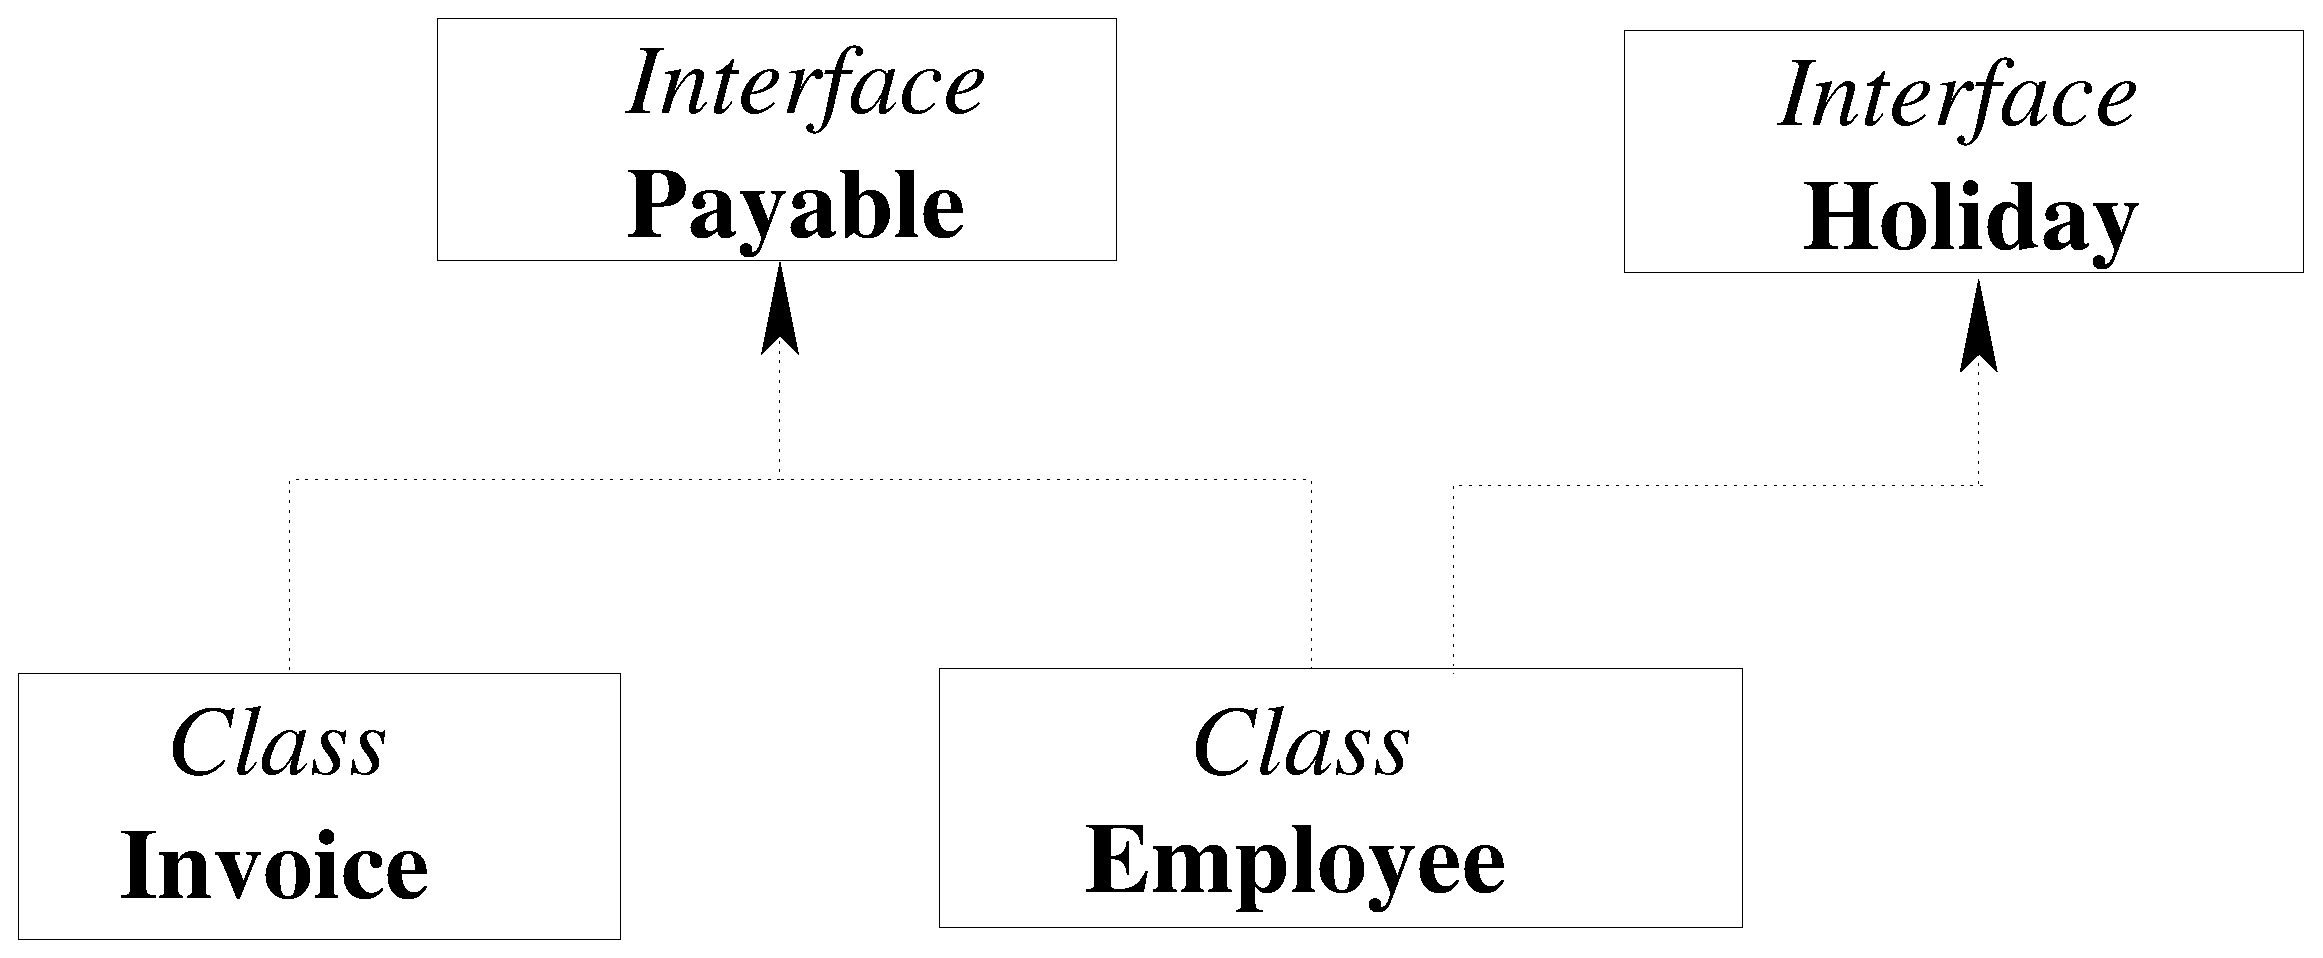
\includegraphics[height=.4\textheight]{structure}
\end{center}

\end{frame}
\end{document}

%%% Local Variables: 
%%% mode: latex
%%% TeX-master: t
%%% End: 
